\documentclass[a4paper]{article}
\usepackage[a4paper, margin=2.5cm]{geometry}
\usepackage[utf8]{inputenc}
\usepackage[T1]{fontenc}
\usepackage{graphicx}
\usepackage[english]{babel}
\usepackage{hyperref}
\usepackage{float}
\usepackage{amsthm}
\usepackage{amsmath}
\usepackage{multicol}
\usepackage{wrapfig}
\usepackage{bm}
\usepackage{amssymb}
\usepackage{listings}
\usepackage{minted}
\usepackage{tikz}
\usetikzlibrary{calc,arrows.meta,positioning, automata, shapes}
\usepackage[]{algorithm2e}
\usepackage{paralist}

\hypersetup{
    colorlinks = true,
    citecolor = black,
    urlcolor = blue,
    linkcolor = black,
}
\usepackage[
    backend=biber,
    style=alphabetic,
    citestyle=authoryear
]{biblatex}
\usepackage{csquotes}
\addbibresource{ref.bib}

\newcommand{\question}[2]{
\paragraph{Question #1} -- \textit{#2}

}
\newcommand{\programming}[1]{
\paragraph{Programming} -- \textit{#1}

}

\title{Reinforcement Learning Lab Session 6}
\author{Lars Van Roy}
 
\begin{document}
\maketitle
\section*{General Information}
This lab session will cover all the Reinforcement Learning material from courses 1 to 4. It will be graded lab sessions. You are free to use any content you want regarding the questions, but please refrain from using outside code beyond the previous lab sessions.

It should be doable in 4 hours, but the deadline will be set to Thursday 2nd of April, midnight. As usual, for there on, each day of delay will remove 2.5/10 points from your grade.

\paragraph{Submission} --
You will have to submit both a report and code through Blackboard. Use the code available on the git at \url{http://github.com/Louis-Bagot/RL_Lab/lab_session6} or \url{https://github.com/Rajawat23/RL_Lab/lab_session6}.

Make a copy of this LaTeX document from folder \textbf{report}, and fill it according to the instructions below. Please to not alter this base document, only add your content.

\question{}{Questions will look like this. For questions, write the answer just below where the (your answer here) appears.}
\programming{Programming exercises will look like this. For programming exercises, read the \texttt{instructions.md} of the corresponding section, and then fill in the corresponding TODO flags in the code. If this text asks for a plot, copy the plot output of your code in the document, in the figure space provided (in addition to leaving it in the plots folder in the code). If the text asks for an explanation of the results, write it as you would answer a question.}

\tableofcontents
\newpage

\section{Bandits}
\question{1}{Explain, in a few lines, the k-armed Bandit problem. Give an example of a real-world application, detailing actions and rewards.}
The k-armed bandits can be used for many real-world applications where there are different options that should be compared with each other. For example different kinds of medications used for a common cause. Each bandit could represent a kind of medicine, each action could be equal to handing a person the medicine, and the reward would be based on the effect of the medicine. For example, the reward could be small/negative if the person was still ill, the reward could be big/positive if the person was cured and the reward could be big and negative in case the person has died.

\question{2}{Derive the incremental updates of the Sample 
Average method.}
In order to optimize the computation of these averages, we do not want to store every obtained result continuously, and therefore we want to optimize the formula $Q_{n+1} = \dfrac{R_1 + R_2 + ... + R_n}{n}$ to the formula $Q_{n+1} = R_n + \dfrac{1}{n} (R_n - Q_n)$ as can be seen in Formula \ref{eq:SampleAverage}.

\begin{equation}\label{eq:SampleAverage}
\begin{split}
Q_{n+1} &= \dfrac{R_1 + R_2 + ... + R_n}{n} \\
		&= \dfrac{1}{n} (\sum_{i=1}^{n} R_i) \\
		&= \dfrac{1}{n} (R_n + \sum_{i=1}^{n-1} R_i) \\
		&= \dfrac{1}{n} (R_n + (n-1) \dfrac{1}{n-1} \sum_{i=1}^{n-1} R_i) \\
		&= \dfrac{1}{n} (R_n + (n-1) Q_n) \\
		&= \dfrac{1}{n} (R_n + n Q_n - Q_n) \\
		&= R_n + \dfrac{1}{n} (R_n - Q_n) 
\end{split}
\end{equation}


\question{3}{Explain, with your own words, the difference between Sample Average and Weighted Average methods}
While using Sample Average methods, we calculate average rewards without any difference between newer observations and older observations. This will always converge and is only suitable for constant environments. Weighted Average methods give the option to make the newer observations more valuable than the older observations, via a weight. This weight must be between 0 and 1, and represent the value of the new result in an update of the average. The closer the weight gets to 1, the closer the updated average will be to the new result, when it gets closer to 0, the updated average will get closer to the old average, and only change slowly. Weighted averages are more suitable for constantly changing environments, and will never converge.

\question{4}{Explain the impact of the hyper-parameters of the following algorithms: $\epsilon$ in $\epsilon$-greedy, $c$ in UCB, and $\alpha$ in Gradient Bandit. Use extreme values as examples.}
In \textit{epsilon-greedy} we will try to avoid getting stuck at local maxima that come with exploitation. When purely basing oneself on the greedy algorithm, we will no longer explore as soon as a local maximum is found. To fix this, we will add a \textit{hyper-parameter} $\epsilon$ in \textit{$\epsilon$-greedy}, which will represent the chance to continue exploring, even though we have found a local maximum. When $\epsilon$ is equal or close to 1, we will continue to explore randomly without any regard for previously found data, when $\epsilon$ is very small or equal to zero, it will be close to or equal to the greedy method.

In \textit{UCB} we try to improve the way we randomly select actions in the greedy method. If it is purely random, we do not consider the potential of an action, if you have tried an action many times, the chances are small that the corresponding average reward will change significantly, where if you have only tried an action a couple of times, the average has a very high probability of changing significantly. We will add a factor the average reward which will allow us to be biased towards actions that have not been chosen as often with that factor being $c\sqrt{\dfrac{\text{ln } t}{N_t(a)}}$. It is clear to see that whenever we have tried an action many times, $N_t$ will get very big, and the factor will become very small, we can also see that whenever we have only tried an action a few times, the factor will get very big due to the same reasoning. The \textit{hyper-parameter c} decides how much this factor is taken into account. When c is small or close to zero, the \textit{UCB} algorithm will approach or be equal to the greedy method. When c becomes large we will purely base ourselves on the actions that we have chosen the least number of times, and no longer have any (or much) regard for the actual average obtained reward.

In \textit{Gradient Bandit} we want to learn a numerical preference (called $H_t(a)$ for an action a) for each action. In this method we will attempt to increase the probability of choosing an action, based on the current reward compared to the average reward. If the reward is higher than the average reward, we increase the probability of choosing said action, and decrease it otherwise. The \textit{hyper-parameter} $\alpha$ will decide the rate at which these probabilities change. A small alpha will cause the probability to change slowly, to not at all, in case $\alpha$ is equal to zero. In case $\alpha$ gets very big, the rate at which the probabilities change will be massive, one bad reward, and the probability of choosing that action will plummet. 

\question{5}{Show that the Sample Average method erases the bias introduced by the initialization of the $Q$ estimates. What does this mean for Optimistic Greedy? Show that, despite this, Optimistic Greedy does not work on non-stationary problems.}
The Sample average method is a method that will always converge eventually, and the change in initial value will not change this. It might take more or less steps to converge (depending on the actual value it converges towards) as it converges very slowly, but it will converge nevertheless. 

Since the added functionality of Optimistic Greedy, being the initialization of Q estimates, did not have any effect on the Sample Average method, it means that we need to use a different method for Optimistic Greedy to compute averages. The one method that would be suitable for this would be Weighted Average, as this will never completely converge.

Despite the fact that Weighted Average is suitable for non-stationary problems, Optimistic Greedy is not. Optimistic Greedy is a method that uses an epsilon value equal to 0, which means that we will always exploit and never explore. The reason that Optimistic Greedy works in stationary situations is that it is forced to explore a little bit due to the initial values, as the optimal action might vary at that point. Once the other ones drop below the currently best action, no other actions will be explored. Over time our current maximum might become a local maximum, but this will never be discovered.

\programming{Implement a Sample Average and Weighted Average version of $\epsilon$ greedy on a Non-Stationary k-armed Bandit problem. In order to see results, run the experiment for $10k$ steps, and paste here the resulting performance plot in the Figure \ref{fig:sa_vs_wa} below. Explain your results below.}
(your explanation here)
\begin{figure}[H]
    \centering
    % Change the plot name here:
    \includegraphics[width=8cm]{plots/agent_comparison_perf.png}
    \caption{Comparison: $\epsilon$-greedy algorithm with Sample Average versus Weighted Average updates.}
    \label{fig:sa_vs_wa}
\end{figure}{}

As we can clearly see, the \textit{Weighted Average} method performs better over time than the \textit{Sample Average} method does. 

This is explainable with the fact that \textit{Sample Average} converges over time, where \textit{Weighted Average} does not. \textit{Sample Average} will converge, and it will get stuck on a maximum, where it will stay indefinitely as the n value will get so big to the point that the average never changes. \textit{Weighted Average} however will never converge, and will always continue changing. The environment will change, but the averages will adapt to this and \textit{Weighted Average} has a far higher chance to continue going for the action with the best reward distribution.


\section{Markov Decision Processes}
For questions where a drawing (MDP or diagram) is required, you can use whichever of the following methods:
\begin{itemize}
    \item a (properly cropped and clear) photo of a drawing on paper. Make sure everything is readable.
    \item a tikz diagram, i.e. the plotting tool for LaTeX (if you know how it works. Don't learn for this report otherwise, tikz takes an eternity)
    \item \href{www.mathcha.io}{Mathcha}, which can generate tikz or pngs. (recommended)
\end{itemize}{}

\question{1}{Define a Markov Decision Process, and the goal of the Reinforcement Learning problem.}
A Markov Decision Process is a means to represent environments in a graph format. A process is defined as a 4-tuple (S, A, $P_\alpha$, $R_\alpha$) where
\begin{itemize}
	\item $S$ is a finite set of states
	\item $A$ is a finte set of actions
	\item $P_\alpha(s, s')$ is a probability function that gives the probability that action a leads to state s' starting from state s
	\item $R_\alpha(s, s')$ is a reward function that gives the reward obtained when going from state s' to state s
\end{itemize}

There could be multiple ways to traverse the graph, as there could be many possible actions that can be performed in each state, we will therefore define a policy function that will make the decisions for us. A policy is a function $\pi$ that specifies the desired action for each state. This can be updated/modified while traversing the different states and their corresponding actions, until it converges, at which point we can say that the process of choosing an action becomes deterministic. The ultimate goal is to define your policy in such a way that the average reward gained while following the policy is maximal.

\question{2}{Show that the MDP framework generalizes over Bandits by drawing the Bandits problem as a MDP with reward distributions $r_a$ for each action $a$. Paste your drawing on Figure \ref{fig:bandit_mdp}. Shortly explain your submission.}



\begin{figure}[H]
    \centering
    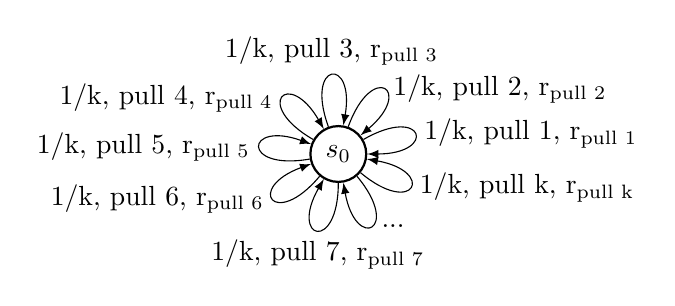
\begin{tikzpicture}[auto,>=latex]    
	    \tikzstyle{round}=[thick,draw=black,circle]
	    
	    \node[round] (s0) {$s_0$};
	    
	    \path[->] (s0) edge [in=0, out=30, looseness=12, right] node {1/k, pull 1, r$_{\text{pull 1}}$} (s0);
	    \path[->] (s0) edge [in=40, out=70, looseness=12, right] node {1/k, pull 2, r$_{\text{pull 2}}$} (s0);
	    \path[->] (s0) edge [in=80, out=110, looseness=12, above] node {1/k, pull 3, r$_{\text{pull 3}}$} (s0);
	    \path[->] (s0) edge [in=120, out=150, looseness=12, left] node {1/k, pull 4, r$_{\text{pull 4}}$} (s0);
	    \path[->] (s0) edge [in=160, out=190, looseness=12, left] node {1/k, pull 5, r$_{\text{pull 5}}$} (s0);
	    \path[->] (s0) edge [in=200, out=230, looseness=12, left] node {1/k, pull 6, r$_{\text{pull 6}}$} (s0);
	    \path[->] (s0) edge [in=240, out=270, looseness=12, below] node {1/k, pull 7, r$_{\text{pull 7}}$} (s0);
	    \path[->] (s0) edge [in=280, out=310, looseness=12, right] node {...} (s0);
	    \path[->] (s0) edge [out=320, in=350, looseness=12, right] node {1/k, pull k, r$_{\text{pull k}}$} (s0);
    
    \end{tikzpicture}
    \caption{The MDP corresponding to the Bandit problem with reward distributions $r_a$, $\forall$ actions $a$}.
    \label{fig:bandit_mdp}
\end{figure}{}
The MDP displayed in Figure \ref{fig:bandit_mdp} describes a means in which the bandit problem can be described. Each transition symbolizes the pulling of a single arm, which comes with the reward of that arm, given by the reward distributions $r_a$, $\forall$ actions a. The chances of each action occurring are uniformly distributed.


\question{3}{Turn the following statement into a MDP, with states and transitions with actions (named), probabilities and rewards. Paste the graph on Figure \ref{fig:q3}; pick real values for both rewards and probabilities (no unknowns). Shortly explain your submission after the statement and plot.}

Statement:

\texttt{You go to the university using Velo -- Antwerp's shared bikes. There are three stations where you can drop off your bike on the way: the park, furthest from the university; the cemetery, second furthest; and the university station, right in front of your destination.
You want to take the least time possible to go to the university, and you take much longer walking than biking. \\
At any station, you can either decide to drop off your bike and walk to the university, or continue to the next station.
However, it sometimes happens that the stations are full - you cannot drop off your bike there. You can either go back, or, if possible, continue.\\
You notice that the amount of free spots in the first stations often aligns with the amount of free spots in the following stations - or is less. In order to decide whether you should drop off your bike or not, you take note of the last station's number of free spots - it can either be a lot, or a few, or none.\\
When you have to go back, we assume that people could've come to pick or drop bikes, so the transition doesn't depend on the previous state of the station.
}

\begin{figure}[H]
    \centering
    % Change the plot name here:
    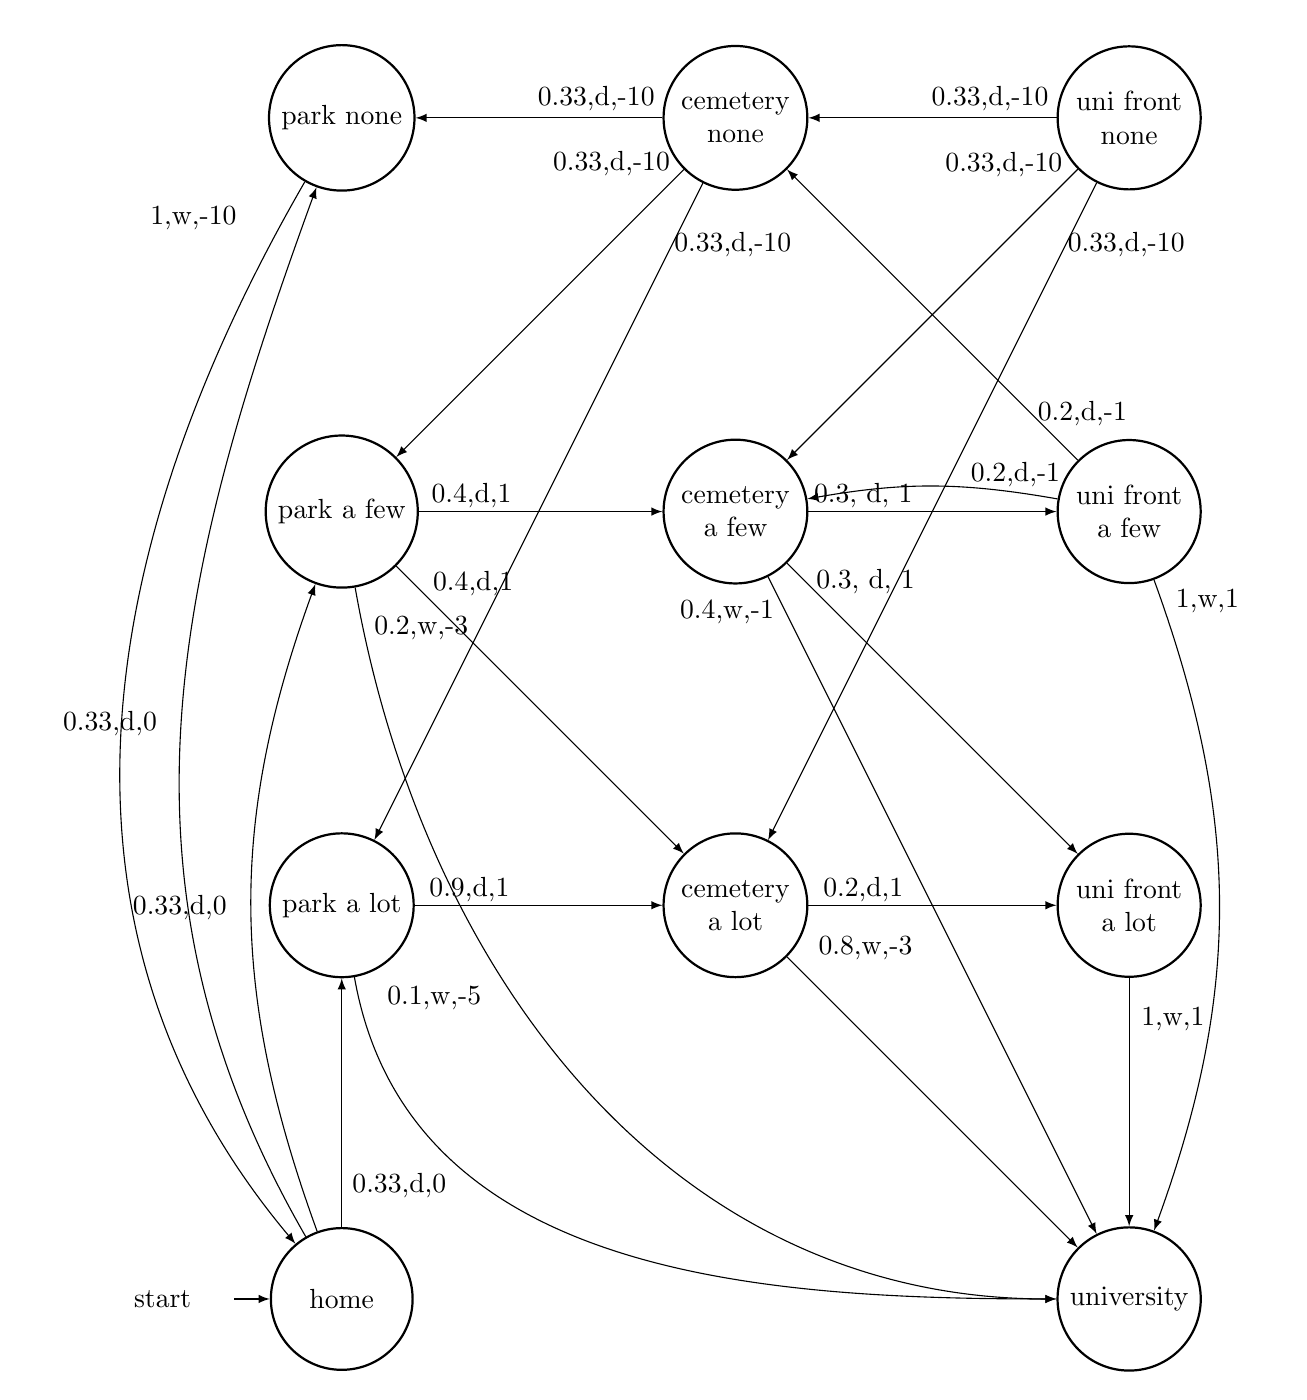
\begin{tikzpicture}[auto,>=latex, node distance=5 cm, minimum size=1.8 cm]    
	    \tikzstyle{round}=[thick,draw=black,circle]
	    
	    \node[round, initial] (home) {home};
	    \node[round] (park a lot) [above of=home] {park a lot};
	    \node[round] (park a few) [above of=park a lot] {park a few};
	    \node[round] (park none) [above of=park a few] {park none};
	    \node[round] (cem a lot) [right of=park a lot, align=center] {cemetery \\ a lot};
	    \node[round] (cem a few) [right of=park a few, align=center] {cemetery \\ a few};
	    \node[round] (cem none) [right of=park none, align=center] {cemetery \\ none};
	    \node[round] (uni a lot) [right of=cem a lot, align=center] {uni front \\ a lot};
	    \node[round] (uni a few) [right of=cem a few, align=center] {uni front \\ a few};
	    \node[round] (uni none) [right of=cem none, align=center] {uni front \\ none};
	    \node[round] (university) [below of=uni a lot] {university};
	    
	    \path[->] 
	    (home) 			edge 					node [right, yshift=-30pt, xshift=-5pt] {0.33,d,0} (park a lot)
	    (home) 			edge [out=110, in=250] 	node [left] {0.33,d,0} (park a few)
	    (home) 			edge [out=120, in=250] 	node [left] {0.33,d,0} (park none)
	  
	    (park a lot)  	edge 					node [yshift=-20 pt, xshift=-25pt] 	{0.9,d,1} (cem a lot)
	    (park a lot)  	edge [out=280, in=180] 	node [yshift= 65 pt, xshift=-90pt] 	{0.1,w,-5} (university)
	    (park a few)  	edge 					node [yshift=-20 pt, xshift=-25pt] 	{0.4,d,1} (cem a few)
	    (park a few)  	edge 				 	node [yshift= 20 pt, xshift=-50pt]	{0.4,d,1} (cem a lot)
	    (park a few)  	edge [out=280, in=180] 	node [yshift=140 pt, xshift=-85pt]	{0.2,w,-3} (university)
	    (park none) 	edge [out=240, in=130] 	node [yshift=210 pt, xshift=-0pt] 	{1,w,-10} (home)
	    
 	    (cem a lot)  	edge 					node [yshift=-20 pt, xshift=-25pt] 	{0.2,d,1} (uni a lot)
	    (cem a lot)  	edge 				 	node [yshift= 30 pt, xshift=-50pt]	{0.8,w,-3} (university)
	    (cem a few)  	edge 					node [yshift=-20 pt, xshift=-25pt] 	{0.3, d, 1} (uni a few)
	    (cem a few)  	edge 				 	node [yshift= 20 pt, xshift=-50pt]	{0.3, d, 1} (uni a lot)
	    (cem a few)  	edge 				  	node [yshift= 80 pt, xshift=-100pt]	{0.4,w,-1} (university)
	    (cem none)	 	edge 					node [yshift=175pt, xshift=-5pt]	{0.33,d,-10} (park a lot)
	    (cem none)		edge					node [yshift= 80pt, xshift= 0pt]	{0.33,d,-10} (park a few)
	    (cem none) 		edge					node [yshift=-20pt, xshift= 70pt]	{0.33,d,-10} (park none)
	    
	    (uni a lot)		edge 					node [yshift= 30pt, xshift=-10pt]	{1,w,1} (university)
	    (uni a few)		edge [out=290, in=70]	node [yshift=110pt, xshift=-30pt]	{1,w,1} (university)
	    (uni a few) 	edge [out=170, in=10]	node [yshift=30pt, xshift=30pt]		{0.2,d,-1} (cem a few)
	    (uni a few) 	edge 					node [yshift=-10pt, xshift=80pt]	{0.2,d,-1} (cem none)
	    (uni none)	 	edge 					node [yshift=175pt, xshift=-5pt]	{0.33,d,-10} (cem a lot)
	    (uni none)		edge					node [yshift= 80pt, xshift= 0pt]	{0.33,d,-10} (cem a few)
	    (uni none) 		edge					node [yshift=-20pt, xshift= 70pt]	{0.33,d,-10} (cem none)
	    ;
    
    \end{tikzpicture}
    \caption{The MDP corresponding to the statement of Question 3}.
    \label{fig:q3}
\end{figure}{}
There are 5 base states, of which 3 have 3 additional substates. There is home, which represents the start of the path, there is park, which is the first station, cemetery, which is the second station and university front, which is the final station. There is one more state which is university, which is the final destination of the biker. The three stations consist out of three substates, where they can either be in completely filled state, defined by none, a partially filled state, defined by a few and mostly empty, defined by a lot.

The transitions from a degree of filled, to the next station, is considered to be random, that is, the filled degree must at least be as high as the previous degree, and the distribution between the leftover options is assumed to be uniform.

The biker favors moving forward, as long as there are spaces left in the current station, as soon as there are none, the biker will always return, and in case the front of the university is reached, the biker will always go for the university (given that there is any space at all). If there is no space in any of the stations, the biker will go back to the previous station, or in case there is no space at the park, the biker will go back home. There is no specification for what happens if none of the stations have spaces, so the decision was made to let the biker return home in this case.

In case a station was filled, the degree of filled from the previous station is considered to be uniformly distributed, and therefore, the chances will be 33\% for each of the previous station's substations.

The rewards are based on the distance traveled by bike. moving forward from station to station will always result in a reward of 1, moving from the front of the university to the university will also result in a reward of 1. Moving back to a previous station will result in a reward of -10, as this should be avoided at any cost, as this is very counter productive. Early transitions from a station to the university will yield negative rewards, based on the closeness to the university, and the number of free spaces. These are less negative than backtracking (as they are less bad) but are still negative, as continuing forward must be better (in case those stations are not packed).

\question{4}{RL has been widely popular lately because of its combination with Deep Learning (using Neural Nets as policy or value function approximators), leading to incredible performances on difficult environments like video games. One such game is the first Mario World. Show how the MDP can look like for the frames of the game. Where can stochasticity be involved?}

Based on a frame, a MDP could be created, to determine the next move of Mario. For example, depending on the closeness of the nearest enemy, a very bad score could be given for walking towards said enemy. Depending on the closeness of the nearest coin, a good score could be given for walking towards said coin. Powerups could be given higher scores than coins and good scores could be decreased in case there are enemies nearby.

In case one wishes to combine this with Neural Nets, stochasticity is necessary as this allows us to explore different possibilities, see how each possibility fares, and learn things from those results.
\section{Control}
In lab session 2 and 3, the Value Iteration algorithm was stopped after a maximum number of iterations. However, this is not the natural stopping condition of the algorithm: it should stop when the value estimates have converged: $V_k = v*$. When implementing this, we define convergence of the $V_{k-1},V_k,V_{k+1}..$ stream of vector values as $$ \vert\vert V_{k+1} - V_k \vert\vert_2 < \delta $$
Where $\delta$ is an arbitrary small constant ($\delta = 0.01$ in the code). The number of iterations of Value Iteration to convergence is a measure of the algorithm's performance.\\

Policy Iteration alternates evaluating a policy $\pi$ until convergence to $V_\pi$, and updating the policy to be greedy over the new values, $\pi ^\prime = greedy(v_\pi)$. We define \textit{convergence in policy} as  $\pi^\prime = \pi$ (same action in all states), and \textit{convergence in value} as $$ \vert\vert V_{\pi ^\prime} - V_\pi \vert\vert_2 < \delta $$

Value Iteration only converges in value, as there is no explicit policy. When comparing convergence speed in value of Value Iteration vs Policy Iteration, make sure to compare the number of single sweeps over the state space! (iterations)

\programming{Implement Value Iteration on the course's diamond/pit Gridworld environment (course and Lab session 2). You can reuse Environment code from before.}

\programming{Implement Policy Iteration on the course's diamond/pit Gridworld environment.}

\question{1}{Discuss and compare the performances of both algorithms. Under what circumstances can one come on top of the other?}

When looking at performance metrics as mentioned in the code, which is based on the number of loops, the Policy Iteration performs worse than the Value Iteration algorithm did, due to Policy Iteration needing additional loops to evaluate the policies. However, these loops are not exactly equal. In the value evaluation loop, Policy Iteration will only need to evaluate one action (being the current policy) per state, where Value Iteration will need to evaluate every action.

In general for complex environments, Policy Iteration will perform better than Value Iteration, Policy Iteration will require us to only compute one action for each states. There might be more loops, since we only consider one of the actions for each state per iteration, but on the other hand the policy will converge faster than the values do. So as soon as the policy stops changing the Policy Iteration will end while the Value Iteration might still carry on. Whenever we consider more simple environments, Value Iteration will be better, since there will only be a small amount of iterations and in those situations, the additional loops required to updates policies etc, could become significant for the total execution time.

\question{3}{Explain the fundamental differences between QLearning and the Value Iteration / Policy Iteration algorithms. Can you see why QLearning is more interesting in the general case?}

The fundamental difference between QLearning and Value Iteration / Policy Iteration, is that in QLearning it is assumed that we have zero knowledge regarding state transition probabilities or rewards. In Value Iteration / Policy Iteration we assume that these things are known. To be able to let the agent work on general cases, it is therefore prudent to use QLearning over Policy Iteration / Value Iteration as we will not have the needed information to perform these.

\section{Bonus}
\programming{\textbf{BONUS, 1.5pts} Implement the Gridworld drawn on Figure \ref{fig:river_crossing}: a river crossing. The actions are up, down, left, right and "do nothing". The agent needs to cross a river from the lower left corner (state S) to the upper right corner (state G). This $3\times 5$ Gridworld is divided on the 2nd row by a river that might push the agent right upon entering by one, two or three squares, with corresponding probabilities $0.2, 0.5$ and $0.3$. If the agent is pushed off to the far right in the river, the episode ends with reward $-1$. If the agent reaches the goal, the reward is $+1$. Note that it is the transition to the state (i.e. "right" from (0,3) to G=(0,4)) that yields the reward, and states G and red (1,4) are terminal. }

\begin{figure}[H]
    \centering
    % Change the plot name here:
    \includegraphics[width=6cm]{plots/river.png}
    \caption{The River Crossing MDP}.
    \label{fig:river_crossing}
\end{figure}{}

Note: By mistake I originally added the specified environment to the code of the third assignment, this code does work, but in order to be fully correct I also implemented this in the requested bonus directory. At this point I am uncertain as to what I changed in order to implement the grid in the third assignment, so I decided to leave this in. Nothing was changed to the rest of the code, but I want to make the remark, in case you check for differences with the original files.


\printbibliography
\end{document}

